\section{Experiments}
\label{sec:experiments}

\subsection{Setup}

We fine-tune Qwen-2.5-7B-Instruct with LoRA \citep{hu2022lora,dettmers2023qlora} on 8K multi-turn conversations from the UltraChat \citep{ding2023ultrachat} training split. Training uses 3 epochs with AdamW (lr $= 2 \times 10^{-4}$, batch size 1, gradient accumulation 8, seed 42; ThreadGate additionally with seed 123); each variant requires approximately 6 hours on a single NVIDIA RTX PRO 6000 Blackwell Server Edition GPU (96\,GB; training costs in Appendix~\ref{sec:appendix-cost}). Full hyperparameters are in Appendix~\ref{sec:appendix-hyper}; dataset statistics in Appendices~\ref{sec:appendix-data} and~\ref{sec:appendix-dataset-ext}; the controlled comparison design is described in \S\ref{sec:comparison-design}. We evaluate under \emph{IID} (same-distribution UltraChat text) and \emph{held-out} (50 non-overlapping conversations) teacher-forced protocols, reporting GAR-ours, GAR-Dongre \citep{dongre2026attention}, and perplexity (PPL).

\subsection{Main Results}

Table~\ref{tab:five-way} presents the five-way comparison. Under TF evaluation, all fine-tuned variants converge: GAR-ours spans 0.49--0.51 ($\leq$2\,pp), PPL is 2.62--2.78. IID and held-out protocols produce identical rankings (held-out GAR-ours differs by $\leq$2\,pp), ruling out data overlap as a confound. GAR-Dongre remains low (0.01--0.02) with no TF-AR gap, indicating that only concentrated last-token attention is vulnerable to distribution shift; scheduled sampling breaks this pattern (\S\ref{subsec:ss}).

Under AR generation ($N$\,=\,50), GAR-ours drops to 0.019--0.064, an 8--17$\times$ gap (Figure~\ref{fig:headline}). The ordering (ThreadGate 0.064 $>$ LoRA-only 0.037 $>$ Uniform Gate 0.033 $>$ PCGrad 0.030 $>$ Base 0.019) shows ThreadGate vs.\ LoRA-only is significant ($p$\,=\,0.004; Appendices~\ref{sec:appendix-stats} and~\ref{sec:appendix-stats-ext}), yet the gap remains 7.9$\times$. A second seed confirms TF stability ($0.504\pm0.001$). MMLU 5-shot accuracy remains within 0.8\,pp across all variants (per-category breakdown in Appendix~\ref{sec:appendix-mmlu-ext}). We analyze this distribution shift in \S\ref{sec:analysis}.

\begin{figure*}[!t]
  \centering
  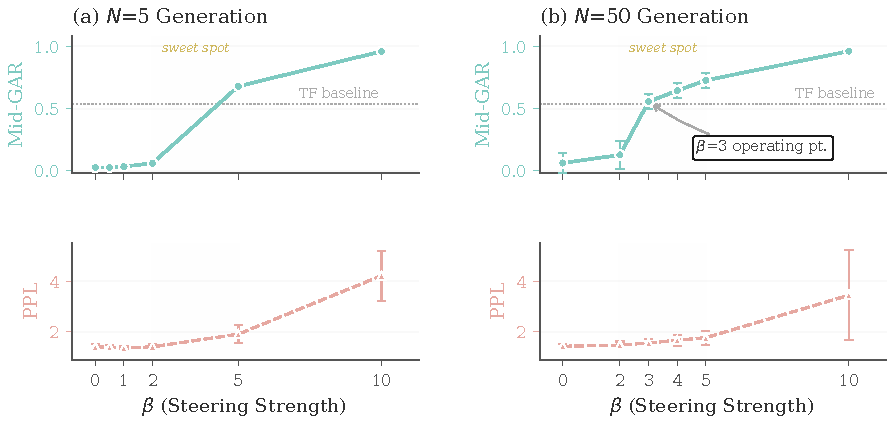
\includegraphics[width=\textwidth]{fig5_attention_steering.pdf}
  \caption{Inference-time $\beta$-steering recovers GAR from 0.064 to 0.727, consistent with attention misallocation as a proximal cause (9\% PPL cost at $\beta$\,=\,3; phase transition at $\beta \in [2, 3]$).}
  \label{fig:steering-recovery}
\end{figure*}

\subsection{Inference-Time Attention Steering}\label{subsec:steering}

All training-time interventions leave the exposure bias gap intact. If the collapse is caused by attention misallocation rather than representation degradation, then directly correcting attention should recover GAR. We test this by adding a constant bias $\beta$ to pre-softmax attention logits for goal-token positions during generation:
\begin{equation}
  \tilde{A}_{i,j}^{(\ell,h)} = A_{i,j}^{(\ell,h)} + \beta \cdot \mathbf{1}[j \in \mathcal{G}],
\end{equation}
where $\tilde{A}$ denotes the modified logits before softmax. The additive form operates in log-probability space, providing uniform boost even when baseline attention is near zero. The response is sharply nonlinear: $\beta \in [0, 2]$ yields marginal improvement, then $\beta = 3$ triggers a phase transition to GAR\,=\,0.556 (9\% PPL cost). At $\beta$\,=\,5, GAR reaches 0.727$\pm$0.061 (PPL 1.77); the operating region $\beta \in [3, 5]$ exceeds the TF baseline while PPL remains below 1.8 (Figure~\ref{fig:steering-recovery}; full results in Appendix~\ref{sec:appendix-steering}; per-$\beta$ turn-level trajectories in Appendix~\ref{sec:appendix-steering-viz}). GAR recovery under steering is partly by construction: boosting attention logits toward goal tokens mechanically increases the attention-based metric. The stronger evidence is the counterfactual: if the collapse were due to hidden-state drift rather than attention misallocation, reweighting could not recover GAR, yet it does, consistent with attention misallocation as a proximal cause (qualitative examples in Appendix~\ref{sec:appendix-examples}). Downstream, steering ($\beta$\,=\,3) raises late-turn instruction compliance by +11.1\,pp, though this effect does not reach conventional significance ($p$\,=\,0.077; content-constrained tasks benefit most, +23.8\,pp; Appendix~\ref{sec:appendix-ir}).

\subsection{Scheduled Sampling Compresses the TF--AR Gap}\label{subsec:ss}

\begin{figure}[t]
  \centering
  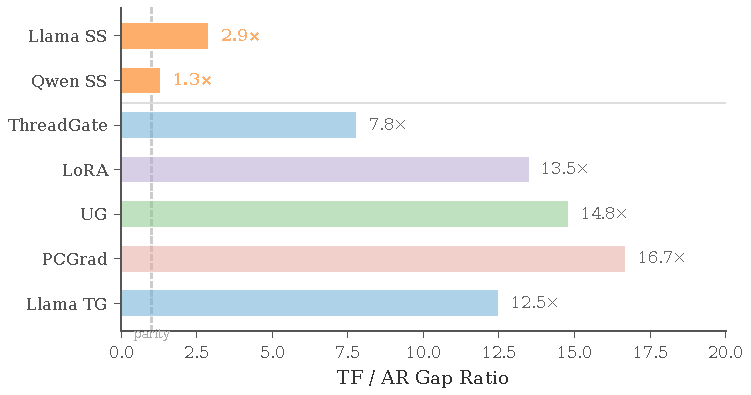
\includegraphics[width=\columnwidth]{fig_ss_gap_compression.pdf}
  \caption{Scheduled sampling compresses the TF-AR gap from 7.9$\times$ to ${\sim}$1.3$\times$ (3-seed mean), the only variant approaching parity across five training conditions.}
  \label{fig:ss-gap}
\end{figure}

Scheduled sampling (SS; \citealp{bengio2015scheduled}), which mixes model-generated tokens into training prefixes with linearly increasing probability (Appendix~\ref{sec:appendix-ss}), directly targets the training-inference mismatch. Across three seeds, AR GAR-ours rises to $0.401\pm0.047$, compressing the gap from 7.9$\times$ to ${\sim}$1.3$\times$ (TF GAR $0.517\pm0.032$; 3-seed mean) with no PPL cost ($1.441\pm0.002$; Figure~\ref{fig:ss-gap}; per-seed details in Appendix~\ref{sec:appendix-perseed}). Steering on SS models nearly eliminates seed variance ($\beta$\,=\,5: $0.717\pm0.001$, std 0.047$\to$0.001; Figure~\ref{fig:ss-multiseed}). SS generalizes across GAR definitions (mid-turn GAR above 0.36 for all token-position variants; Appendix~\ref{sec:appendix-gar-robust}; extended robustness in Appendix~\ref{sec:appendix-gar-ext}) and across architectures: on Llama-3.1-8B, SS compresses the gap from ${\sim}$27$\times$ to 2.9$\times$, weaker than Qwen likely due to fewer training epochs (2 vs.\ 3; \S\ref{subsec:cross-model}). The benefit diminishes in longer dialogues (Appendix~\ref{sec:appendix-n5}), consistent with exposure bias compounding over turns.


